\chapter{PACOTE DE VALOR}
\label{chap:pacotedevalor}

O pacote de valor é definido como sendo um conjunto de bens e serviços fornecidos, em variadas proporções, para os clientes. Desta forma as empresas que prestam serviços ou fornecem produtos passam a fornecer outros itens que agregam e consolidam as relações com seus clientes.
Apesar do pacote de valor fortalecer essas relações é necessário que as empresas expandam os mesmos fornecendo mais benefícios aos clientes.
Para se produzir o pacote de valor o processo é semelhante à produção de produto, como descrito na Figura \ref{fig:pacotevalor}.

\begin{figure}[H]
    \caption{Fluxo da geração do pacote de valor.}
    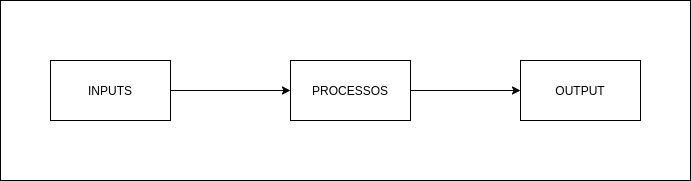
\includegraphics[width=\textwidth]{images/pacote_valor.png}
    \label{fig:pacotevalor}
    \caption*{Fonte: baseado no Slack, 2006.}

\end{figure}

Os inputs podem ser divididos em: recursos a serem transformados (matérias-primas, informações e clientes) ou recursos de transformação (instalações e prédios, máquinas e equipamentos, e empregados). Os processos englobam o projeto, planejamento e controle, melhorias e estratégias de produção. E como output tem-se os bens e serviços, ou seja, o pacote de valor \cite{slack2006administraccao}.
%------------------------------------------------------------------
\section{Aplicação Prática}
\label{sec:app1}
O pacote de valor da empresa SunBurn revolve entorno da produção e venda de energia elétrica, bem como serviços agregados. No território nacional, esta empresa produz energia elétrica através da produção solar e eólica, a qual é fornecida para empresa distribuidora regionalmente instalada. 

Acredita-se que o pacote de valor da empresa pode ser expandido através da integração das tecnologias de produção de forma que ela possa garantir o fornecimento da energia que vende mesmo quando algum incidente ocorra na geração através de uma das tecnologias. O atual uso de diferentes fontes limpas de energia aumenta deve apenas ser realizado de forma integrada de forma a criar uma redundância do sistema de produção da Sunburn. Esta integração pode então ser vendida como um serviço adicional de aumento na garantia da entrega de energia para o cliente.

A SunBurn já possui um estudo para a formação de micro-geradoras de energia elétrica, as quais são implantadas direto no cliente final. Tal modo de produção viabiliza a redução dos custos agregados na transmissão e distribuição de energia elétrica para o cliente, além de possibilitar uma redundância local no fornecimento de energia para o cliente em questão. Esse modo de geração de energia, poderá ser amplamente utilizado pela SunBurn após a regulamentação local da venda de energia elétrica produzida por essas micro-geradoras para as empresas de transmissão e distribuição. A SunBurn poderá oferecer os seus serviços de regulação, controle e manejo do fornecimento de energia para os seus clientes que possuam usinas micro-geradoras, de forma que os clientes possam vender o excedente de energia gerado em seus territórios.



% \subsection{Requisitos do cliente}
% \label{sub:reqc}
